%!TEX TS-program = xelatex
%!TEX encoding = UTF-8 Unicode
\documentclass[11pt, a4paper]{book}
\usepackage{my-additions-x}

% my macros
\def\code{\texttt}
\def\tred{\texttt{TrEd}}
\def\ntred{\texttt{N-TrEd}}
\def\seman{\texttt{SemAnn}}
\def\semlex{\texttt{SemLex}}
\def\astst{$\ast$.st}
\def\sdata{s-data}
\def\tdata{t-data}
\def\stn{st-node}
\def\sn{s-node}
\def\tn{t-node}
\def\stf{st-file}
\def\sf{s-file}
\def\tf{t-file}
\def\mwe{MWE}
\def\Mwe{multi-word expression}
\newcommand\Sref[1]{Section~\ref{#1}}

\title{Thesis Notes}
\author{\textsc{Pavel Straňák}}

\begin{document}
\maketitle

%%%%%%%%%%
\section*{Motto}
\begin{tabular}{@{} lp{11cm} @{}} % @{} removes default spaces
Frasier: & ``How was your hunting trip?''\\
Martin: & ``Came home empty handed.''\\
Frasier: & ``Oh dear; I guess that means for the next several weeks we'll hear your grouse about the grouse and carp about the carp.''\\
Niles: & ``You've been working on that, haven't you?''\\
Frasier: & ``Well, there was traffic.''\\
 & \raggedleft\emph{Frasier, Season 9, Part 3}\\
\end{tabular}



\newpage
\section{Notes}

{\em``Prokopnout pětku''} -- prokopnout [trestný kop after scoring] pětka -- ellipsis crossing into pragmatics(?), because it is {\em not} an ellipsis of some exact linguistic construction, but rather an ellipsis of a situation which everyone in the discourse understand.  

``Návrh / novela Zákona na ochranu osobních údajů''  $$((\mathrm{návrh} \lor \mathrm{novela}) | \mathrm{zákon} \lor \mathrm{předpis})$$
-- lexikální funkce?? \citep{melcuk:1992} ?

\subsection{Missing t-nodes in \code{coord}s}
``\textit{První} a druhá světová válka'' apod. -- the word ``První'' is an ellipsis of ``První světová válka''. The ellided t-nodes that should had been newly established were not, however, which left us with two options: either annotate a single-word (and single-node) expression as an instance of a multi-word lexeme, or annotate the words ``světová válka'' that occure in the text as being a part of both expressions. We decided for the first, because the agreement on ellipses is fairly high in this type of coordinations.

% !TEX root = ../disertace.tex
%!TEX encoding = UTF-8 Unicode

\chapter{Idioms}
Even ``non-compositional'' idioms are actually (originaly) metaphorical or methonymical.  Even though sometimes it is hard to see that. At other times a speaker may forget that rather straightforward metaphoric aspect:

\begin{quote}
Barack Obama accused his Republican rivals of stirring a controversy over a comment he made about putting “lipstick on a pig.” \emph{(NY~Times, 11.~September 2008)}
\end{quote}

\section{Sinclair}
Patrick Hanks gives a very succinct introduction to John Sinclair's \citep{sinclair:wiki} view of a lexical unit and meaning distinctions. It is closely related to Hanks' own work, as we cen see in \citet{hanks:norms}.

\section{Žabokrtský}
Zdeněk Žabokrtský defines a \emph{lexeme} in his doctoral thesis \citep{zabokrtsky:2005a}, as well as several other basic concepts that he requires for precise description of his work on valency lexicon of Czech verbs. His definition is based on the concept of lexeme as defined in works of \citet{cermak:91} and \citet{filipec:1994} and a concept of lexical unit as defined by \citet{cruse:1986}\footnote{Žabokrský cites \citealp{verspoor:1997}'s description of Cruse's lexeme, but that makes no diference {\xxx(check!)}}. Žabokrtský's view seems to differ from the view of the above mentioned authors, but that difference deserves some analysis.

Žabokrtský defines a lexeme as ``an ordered pair which couples the set of lexical forms and the set of lexical units''. This way a definition of lexeme is based on a definition of the concepts ``lexical form'' and ``lexical unit''. It is also implied that these are somehow complementary. 

A lexeme is however a relativelly common concept in lexicography. It has been defined at least by Lyons, by Cruse, Čermák, Filipec, and probably by many other authors. What is common to all of these definitions is that they construe lexeme as a unit consisting of some lexical form and meaning. 
\emph{It is in fact interesting to try to find what distinguishes a concept of lexeme from a concept of concept itself! It seems that a conncept is also a meaning (essentia) with a form.} See \citet{materna:1998,stranak:2001} for detailed discussion of definition of concepts as well as thorough explanation (in the latter) of the reasons why we do not delve into the problem of concept itself too deeply: it is out of the methodological reach of modern science as we understand it: the problem of what is a concept cannot be solved by any conceptual analysis.

A \emph{lexical unit} in turn is used as defined by Verspoor referring to \citet{cruse:1986}.\footnote%
{\xxx Najit Crusovu definici lexemu a lex. unit a analyzovat. Ma tam MWE, nebo NE??} 

%%%%%
\section{MWE}

\citet{baldwin:2004} defines MWEs very broadly as entities that are:
\begin{itemize}
\item
``decomposable into multiple simplex words,'' and
\item
``lexically, syntactically, semantically, pragmatically and/or statistically idiosyncratic.''
\end{itemize}

His examples are as follows: \emph{``San Francisco, ad hoc, by and large, Where Eagles Dare, kick the bucket, part of speech, in step, the Oakland Raiders, trip the light fantastic, telephone box, call (someone) up, take a walk, do a number on (someone), take (unfair) advantage (of), pull strings, kindle excitement, fresh air, \ldots''}

From the definition and the examples it is clear that Baldwin includes not only idioms and complex verbs, but also any named entities and even any statistically or pragmatically important\footnote{We avoid a MWE (sic!) ``statistically significant'' on purpose, because we assume that Baldwin also avoids it on purpose when using a word ``idiosyncratic''. As far as we know ``statistically idiosyncratic'' is not a well defined term byt we understand it as saying that not any statistically significant difference in distribution is peculiar enough to be called ``idiosyncratic''. We are fully aware how imprecise this sounds.} collocations. At least that is what we understand as ``statistically idiosyncratic''. Such expressions include ``environmental policy'' but also ``salt and pepper'', which is semantically quite compositional and simple, but statistically the order of its components is significant. In the Corpus of Contemporary American English (COCA, \url{http://www.americancorpus.org/}), there are 3648 occurrences of ``salt and pepper'' vs. 62 occurrences of ``pepper and salt''. Of the 62 occurrences 60 are in recepies. This is rather extreme case of ``statistical idiosyncracy''; as such it well illustrates the point.

Such a broad definition basically says that MWEs are ``interesting collocations'' but in its broadness it is not suitable for our purpose. Since we base our work on the comcept of (monosemic) lexeme, we are more interested in the more conventional approach that Baldwin has in most of his other (co-authored) papers \citep{baldwin:2003,sag:2002}. MWEs are viewed as ``cohesive lexemes that cross word boundaries''. This seems to be the most common definition of MWEs in NLP, as long as we abstract from subtle differences in terminology \citep{calzolari, copestake, dalsi?}. {\xxx je to taky shodne s tradicnimi lingvisty? Cruse? Lyons? cesti?}


\section{ToAdd}
Pecina, Cruse, Filipec, Čermák (rozdelit, nebo spojit se ZŽ?), Hanks. Zminit clanek SC, MH a Lenky?? o Hanksove CPA jako realizaci Sinclairova pristupu k lexikalnimu vyznamu.

Valencni slovniky a \emph{anotace valence}.
% !TEX root = ../disertace.tex
%!TEX encoding = UTF-8 Unicode

\chapter{How are things in PDT 2.0}\label{PDT}
\label{sec:pdt}
\section{Prague Dependency Treebank}
\label{sec:pdt/pdt}
We work with the Prague Dependency Treebank (PDT, see \citealp{hajic:2005}), which is a large corpus with rich annotation on three layers: it has in addition to the morphological and the surface syntactic layers also the tectogrammatical layer.
(In fact, there is also one non-annotation layer, representing the ``raw-text'' segmented into documents, paragraphs, and tokens.)
Annotation of a sentence on the morphological layer consists of attaching several attributes to the tokens of the w-layer, the most important of which are morphological lemma and tag.
A sentence at the analytical layer is represented as a rooted ordered tree with labeled nodes. The dependency relation between two nodes is captured by an edge with a functional label.
The tectogrammatical layer has been construed as the layer of the (literal) meaning of the sentence and thus should be composed of monosemic lexemes and the relations between their occurrences.%
\footnote{With a few exceptions, such as personal pronouns (that refer to other lexeme) or coordination heads.}

On the tectogrammatical layer only the autosemantic words form nodes in a tree (t-nodes). Synsemantic (function) words are represented by various attributes of t-nodes. Each t-node has a lemma: an attribute whose value is the node's basic lexical form.
Currently t-nodes, and consequently their t-lemmas, are still visibly derived from the morphological division of text into tokens. This preliminary handling has always been considered unsatisfactory in FGD.%
\footnote{Functional Generative Description (FGD, \citealp{sgall-etal:1986,hajicova:1998}) is a framework for systematic description of a language, that the PDT project is based upon. In FGD units of the t-layer are construed equivalently to monosemic lexemes and are combined into dependency trees, based on syntactic valency of the t-nodes.}
There is a clear goal to distinguish t-lemmas through their senses, but %so far this process has only been completed for verbs and deverbative nouns and adjectives. 
this process has not been completed so far (see Section \ref{sec:pdt}).

Figure~\ref{fig:layers} shows the relations between the neighboring layers of PDT. 
\begin{figure}[htbp]
   \centering
   \includegraphics[scale=.38]{images/roviny.pdf} %180,0,580,595
%\begin{center}
%\epsfig{file=images/roviny.pdf,height=6cm,bbllx=100,bblly=425,bburx=300,
%        bbury=625,clip=}
%\end{center}
   \caption{The rendered Czech sentence \emph{Byl by šel dolesa}. (lit.: He-was would went toforest.) contains past conditional of the verb ``jít'' (to go) and a typo ``toforest'' repaired on m-layer.}
   \label{fig:layers}
\end{figure}

Our project aims at improving the current state of t-lemmas. Our goal is to assign each t-node a t-lemma that would correspond to a lexeme, i.e. that would really distinguish the t-node's lexical meanings. To achieve this goal, in the first phase of the project, which we report on in this paper, we \emph{identify multiword expressions and create a lexicon of the corresponding lexias}. A simple view of the result of our annotations is given in the Figure~\ref{fig:trees}, some technical details are in Section~\ref{sec:meth:annot}.
%Remaining t-lemmas of ``single-word t-nodes'' will be examined and possibly changed later. But to do that, we must finish the current phase in order to know what the remaining ``single-word'' nodes are.

% to leave out ???
%There are also other quite practical motivations for MWE annotation: If we want to identify coreference relations between for instance ``Association for Computational Linguistics'', ``ACL'', and  ``it'' in a text, we need to identify the first expression as a single unit. For some applications we might also need to know what kind of entity it is. 

\begin{figure}[htbp]
   \centering
   \includegraphics[width=3.4in]{images/stromecky.pdf}
   \caption{Schema of the changes in t-trees after integration of our annotations; every MWE forms a single node and has its lexicon entry}
   \label{fig:trees}
\end{figure}


In the Prague dependency treebank version 2.0 (PDT, ) there are several functors that refer to multiword expressions (MWEs) in one way or another. There are also two technical lemmas \texttt{\#Idph} and \texttt{\#Forn} that identify roots of subtrees representing MWE's. Tectogrammatical annotation is described in detail in~\citet{mikulova:2006}.


\section{Search and visualisation tools}

There are currently two graphical search engines for PDT: Netgraph \citep{mirovsky:2009} and TrEd \citep{pajas:tred}. Both have their respective benefits, but since TrEd is considerably faster due to its use of an SQL database backend \citep{pmltq}, we have used TrEd for all the examples in this work. We also give the search queries using the PML Tree Query language designed by \citet{pmltq} where appropriate.

%%%%%%%%%%
\section{List structures}

\subsection{Foreign Phrase: \code{t-node [t\_lemma = \#Forn]}}\label{PDT:Forn}
Foreign Phrase seems to be overused and its overuse seems a bit arbitrary. \\
- jmena firem jsou nekdy forn, nekdy ne. (dohledat)\\

%%
\subsubsection{Foreign phrases with just one t-node}
There are 34 occurrences of this construction in the PDT~2.0. Counting them is as easy as writing a query in Figure~\ref{fig:tq-forn1} and extending it with this filter: \code{>>count(\$n)}.

\begin{wrapfigure}{r}{0.32 \textwidth}
\includegraphics[width=0.3 \textwidth]{images/vyhledavky/query-forn-1-x.pdf}
\caption{PML-TQ search query for single-node foreing phrases}
\label{fig:tq-forn1}
\end{wrapfigure}

In case of the bibliographic reference in Figure~\ref{fig:forn-biblio} there is coordination of three foreign phrases corresponding to the parts of a bibliographic reference annotated, but the reason for this is not very clear. After all, the point of annotating foreign phrases as simple lists with a \code{\#Forn} node as a head was to make no assumptions about these pieces of a text \pageref{pdt-t-man:300}.  \\
- je to kvuli te interpunkci???

\begin{figure}[h]
\includegraphics[width=\textwidth]{images/vyhledavky/forn-coord1x-biblio.pdf}
\caption{A bibliographic reference analysed as a coordination of three foreign phrases}
\label{fig:forn-biblio}
\end{figure}

Names of companies seem to be distinguished more by the country of origin then by any linguistic reasons, as demonstrated in Figure~\ref{fig:forn-firmy}. As far as linguistic criteria are concerned, Chemapol and Inekon are as foreign as Agip or Total. However the first two are, or at least were,%
\footnote{At the time of writing this thesis Chemapol is owned by another international company, which only emphasises vagueness of this distinction} %
%
Czech companies, while those in the latter group have a foreign origin.

\begin{figure}
\includegraphics[width=\textwidth]{images/vyhledavky/nazvy-firem.pdf}
\caption{Annotation of Czech and foreign company names}
\label{fig:forn-firmy}
\end{figure}

%%%%%%%%%%
\section{CPHR and DPHR}

\subsection{CPHR}
There are 76 occurrences of {\tt CPHR} nodes, whose head verb is not its parent, but only effective parent, in 40 sentences. See Figure~\ref{fig:tq-echild} for the query and Figures~\ref{fig:cphr-echild} and~\ref{fig:cphr-echild2} for examples.
\begin{wrapfigure}{r}{0.32 \textwidth}
\includegraphics[width=0.3 \textwidth]{images/vyhledavky/query-echild.pdf}
\caption{PML-TQ search query for CPHR nodes, whose effective parrent is not its parent}
\label{fig:tq-echild}
\end{wrapfigure}

\begin{figure}[h]
\includegraphics[width=0.8\textwidth]{images/vyhledavky/cphr-echild.pdf}
\caption{Coordination of verbonominal idioms, where the verbal parts are further ???rozvite }
\label{fig:cphr-echild}
\end{figure}

Figure~\ref{fig:cphr-echild2} shows on the other hand a coordination of two V-N idioms with the same verbal part.
\begin{figure}[h]
\includegraphics[width=\textwidth]{images/vyhledavky/cphr-ukladat-sankce-a-penale.pdf}
\caption{Coordination of two idioms starting with the same verb}
\label{fig:cphr-echild2}
\end{figure}


%%%%%
\section{JLRE -- Current state of MWEs in PDT 2.0}
\label{sec:pdt}
%
%\subsection{Multiword Expressions}
%\label{sec:pdt-mwe}

During the annotation of valency, which is a part of the tectogrammatical layer of PDT 2.0, the t-lemmas, have been basically identified for all the verbs and some nouns and adjectives.
The resulting valency lexicon is called PDT-VALLEX \citep{hajic:2003} and we can see it as a repository of lexemes based on verbs, adjectives and nouns in PDT that have valency.
%
\footnote{It is so because in PDT-VALLEX valency is not the only criterion for distinguishing frames (=meanings). Two words with the same morphological lemma and valency frame are assigned two different frames if their meaning differs.} 

This is a starting point for having t-nodes corresponding to lexemes. However in the current state it is not fully sufficient even for verbs, mainly because parts of MWEs are not joined into one node. Parts of frames marked as idiomatic are still represented by separate t-nodes in a tectogrammatical tree (e.g.~nodes with t-lemmas {\tt“co”} in Figure~\ref{fig:co-nevidet} or {\tt“k\_dispozici”} in Figure~\ref{fig:asistent}). Verbonominal phrasemes are also split into two nodes, where the nominal part is governed by the verb. Non-verbal idioms have not been annotated at all in the current state of PDT. 

In Figures~\ref{fig:co-nevidet}, \ref{fig:klaus}, and \ref{fig:asistent} we give several examples of t-trees in PDT 2.0, that include idioms, light verb constructions and named entities:
\begin{figure}[htbp]
   \centerline{\includegraphics[scale=.7]{images/co-nevidet-clause.pdf}}
   \caption{Idiom \emph{Co nevidět} meaning ``in a blink (of an eye)'', (literally: what not-see)}
   \label{fig:co-nevidet}
\end{figure}

\begin{figure}[htbp]
   \centerline{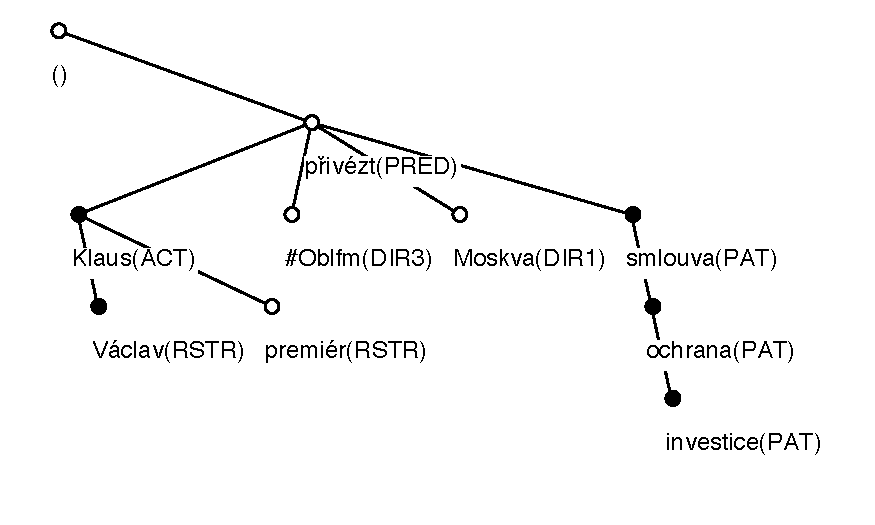
\includegraphics[width=3.7in]{images/klaus-a-smlouva.pdf}}
   \caption{A sentence featuring a personal name and a name of a bilateral treaty (which is not the exact official name, however, thus it is not capitalized)}
   \label{fig:klaus}
\end{figure}

\begin{figure}[htbp]
   \centerline{\includegraphics[height=2.6in]{images/as-pod.pdf}}
   \caption{A t-tree of a sentence featuring a light verb construction \emph{mít k dispozici} (lit.: to have at [one's] disposal) and a named entity (a product name\emph{Asistent podnikatele} (lit.: assistant of-businessman) that looks like a common phrase, except for the capital `A'.}
   \label{fig:asistent}
\end{figure}

%[[!!! doplnit informaci o seznamových strukturách s kořenem \#Idph či \#Forn.]]

% !TEX root = ../disertace.tex
\section{\sdata}
\subsection{The design and the PML schema}
\sdata\ means s-layer PML files and the PML schema of these files. The idea behind \sdata\ design is to have a simple way to store additional ``sense'' annotations over any layer of PDT. The annotations are stored as a set of ``sense'' nodes where each s-node contains a link to a sense repository (annotation dictionary) and a set of references to nodes (m-, a- or t-) that correspond to an instance of the sense. An \sf\ is thus basically a very simple flat list of \sn{}s. It does not contain any trees. A single \sf\ can only reference a single PDT file: either tectogrammatical, or analytical, or even morphological layer can be used, but references to different layer cannot be mixed.

\subsection{Visualisation}
There are two basic ways to view st-nodes: in \seman\ or in \tred. Both of these need to use the ``t-a-m-w-'' PDT files to display the sentence and/or the tree for each sentence and then they read the \stf\ to add the information about \stn{}s. The \stn{}s are displayed as colour boxes or bubbles over the words in a sentence or nodes in a tree in \seman\ or \tred\ respectively.

\subsubsection{\seman}
The visualisation of annotated files in \seman\ has the advantage of showing whole text with all the \mwe{}s in single glance. Integration of the SemLex browser is also beneficial. Details of \seman\ interface are described in \Sref{sec:seman}. 

The drawbacks on the other hand are:
%!TEX root = ../disertace.tex
%!TEX encoding = UTF-8 Unicode

\chapter{\seman}
\label{sec:seman}
The annotation tool \seman\ is written in Perl 5\footnote{\url{www.perl.org}; \url{dev.perl.org/perl5}} with Perl/Tk\footnote{\url{http://search.cpan.org/~srezic/Tk-804.029/}} GUI toolkit. The annotation tool depends on working installation of \tred, specifically its unix installation, because it uses \texttt{nTrEd} for efficient execution of \tred\ scripts in the background. \texttt{nTrEd} however, unlike \tred\ itself or \texttt{bTrEd}, does not work on Windows.% because it uses unix sockets.

% sem-ann screenshot 
\begin{figure}[htbp]
   \centering
   \includegraphics[width=.9\textwidth]{images/sem-ann.png} 
   \caption{An annotated document in \seman. the ``\code{sel}''-- selection tag is barely visible on the word \pr{umění} (second word from the left, second line from the bottom). The \semlex\ entry that is displayed in the Semlex-part of the UI -- \pr{výtvarná umění} -- is the one used to annotate the selected word. }
   \label{fig:seman-gui}
\end{figure}

\seman\ itself is composed of several main parts:
\begin{itemize}
  \item The main application file \code{sem-ann.pl} mostly implements the application frontend. It implements the GUI, loads an \sf, a \semlex,  and a log file for this \sf, if it had already been annotated. Then it takes care of all the interaction with the user and writes \sf, \semlex, and a log file.
  \item \ntred\ backend that is used to 
	\begin{itemize}
	  \item generate surface sentences from tectogrammatical trees in \tf{}s that are then displayed in the \seman\ GUI,
	  \item perform all the on-the fly pre-annotations (\Sref{sec:annot:pre})
	\end{itemize}
	What we call ``backend'' is thus the running \ntred\ instance itself (that is run by the \seman\ during start-up), and the scripts used to generate the sentences that are displayed in \seman\ and to pre-annotate MWEs using their tectogrammatical tree structures.\footnote{these scripts were written entirely by E. Bejček~(\citeyear{bejcek:2010}).}
  \item The module \code{SemLex.pm} is used to read, save, query, and edit \semlex.
    \item The module \code{SemLex\textunderscore{}heslo.pm} implements the \semlex\ entry: its structure, attributes and accessors.
  \item There is also a suite of miscellaneous scripts mostly for validation of annotated data, comparing and merging multiple annotations, merging annotators' \semlex{}es, computing reliability of annotations, and other small tasks related to annotation and managing the annotated data and \semlex{}es.
\end{itemize}

%%%%%%%%%%%%%%%%%%
\section{User interface}
\label{sec:seman:gui}
The user interface (shown in \Fref{fig:seman-gui}) is divided three main parts: The text widget displaying the annotated text, a row of buttons to create annotations by NE tags, show info on annotations, or remove tags, and an editor of \semlex. 



%%%%%%
\subsection{Text widget}
\label{sec:text-widget}
The text, displayed for the annotator, is generated from the tectogrammatical trees (using also information from lower layers). That is, why for each document to be annotated, all the PDT files must be present ( t-, a-, m-, and w-layer). 

It is possible to generate the surface (plain text) sentence from a t-tree using the `built-in' function \verb=PML_T::GetSentenceString($root)=. Such a sentence is complete, correct, has correct spacing around punctuation, but it contains no relation to the t-layer anymore. And we want to keep this connection in order to be able to annotate the t-nodes, not just words \see{sec:annot}. Thus Eduard Bejček wrote the script \url{get_sent_t-layer.btred}, that creates a representation connecting words in a sentence with tectogrammatical IDs of the t-nodes from which these words are generated. This representation is actually input into the text widget and everything but the words is hidden from the annotators' view. \emph{The tecto-IDs are then what gets really annotated, \emph{using} the words.} The full representation can, however, be displayed using Debug menu commands. It is shown in \Fref{fig:seman:hidden} in comparison to the ``plain text'' as normally displayed (with no actual annotations to keep the view simple).

%% comparison of plain text and the same with hidden text -- screenshots%%
\begin{figure}[htbp]
   \centering
   \includegraphics[width=.95\textwidth]{images/hidden-text}
   \caption{Comparison of the plain text, as normally displayed, and the underlying representation that is used to relate the actions of annotators, who mark words, to references to tectogrammatical nodes,that are actually saved in the annotation files.}
   \label{fig:seman:hidden}
\end{figure}



%%%%%%
\subsection{Annotation buttons}
The row of buttons below the text widget and the status bar is rather straightforward: 

The first group (from the left) contains two buttons that are connected to general commands used for all annotations (NEs and other \semlex\ entries alike). The first button shows a tag (i.e. the corresponding \semlex\ entry), on the word in focus (the word that is selected, or in which the cursor is placed). The second button removes the tag on the word in focus.

The second group of buttons simply creates NE tags over the selection. 

The last check button toggles the on-the-fly pre-annotation of other instances of the same MWE that annotator annotates, in the rest of the text (pre-annotation type~\ref{pre-on-annot}, see p.~\pageref{pre-on-annot}).



%%%%%%
\subsection{SemLex editor}
The \semlex\ editor and browser (see the lower part of \Fref{fig:seman-gui}) simply displays SemLex entries, allows to edit them, or to search SemLex by basic or lemmatised forms (see~\Fref{fig:semlex-search}), and browse the search results (using their basic forms). There is also a function to annotate the selected words (t-nodes) with the current SemLex entry. It is mapped simply to the return/enter key, once the focus moves from the SemLex part of the GUI to the text widget.

The attributes of an entry that are displayed include the basic and lemmatised form of an entry, its ID and source, example of usage, synonyms, if present, and a gloss. There is also a time stamp and a signature of the last modification. The attributes of a SemLex entry are explained in detail in \Sref{sec:semlex:entry}.

The search string is by default matched as a substring, and there is a check box to toggle case sensitivity. However when needed (and in case an annotator has the knowledge), full Perl regular expressions can be used. 
\begin{figure}[htbp]
   \centering
   \includegraphics[width=\textwidth]{images/semlex-search}
   \caption{A result of a search in SemLex by a substring of the lemmatised form: 206 entries were found (see the status line at the top). Browsing the basic forms of the results.}
   \label{fig:semlex-search}
\end{figure}

%%%%%%
\subsection{General UI remarks}
Inspired by command mode of modal text editors and by some annotation regimes of \tred, we made all the annotation commands single-letter. That was made possible by making the text read-only. Since the letters are not used for input, they can be mapped to commands. All the command (and so the buttons) are named (in Czech) in such manner, that their first letter can be mapped to perform the command. Only the command for removing annotation is mapped to the capital letter (`O' for `odstranit') for safety reasons.


%%%%%%%%%%%%%%%%%%%
\section{Annotation logs}
\label{sec:logs}
\todo



% !TEX root = ../disertace.tex
\chapter{JLRE paper - rozradit}



%%%%%
%\section{Structure of the Paper}
%\label{sec:structure}

%In Section~\ref{sec:intro} we introduce our annotation task together with some necessary terminology. Section~\ref{sec:pdt} shows the current status of MWEs in the Prague Dependency Treebank, which we work with. Sections~\ref{sec:meth} and \ref{sec:pre} describe our methodology in more detail and Section~\ref{sec:analysis} presents some results, a way to measure agreement on our annotation, and an interpretation of our results.





%%%%%
\section{Methodology}
\label{sec:meth}





% !TEX root = ../disertace.tex
%!TEX encoding = UTF-8 Unicode

\chapter{Conclusions and Future work}
\label{sec:conclusion}

\section{Conclusions}

Several years ago, we were thinking about the best way to begin working on improving the state of t-lemmas: to push them a bit forward, from the legacy of surface layer they still carry, towards deeper representation of lexical meaning. Our conclusion was, partly due to our previous experience with annotation using Czech WordNet as the annotation lexicon \citep{holub:2003,bejcek:2006}, was to start by identifying multiword expressions.

We came forward with two hypotheses based on the properties of dependency syntax and specifically of the tectogrammatical description: 1) That each MWE should form a single contiguous dependency structure, and 2) That all instances of a MWE should share the same dependency structure.

After examining a possibility of annotating t-trees directly we came with an idea of an annotation tool that presents a continuous plain text, but links the plain text to the underlying tectogrammatical structure, from which it is generated. 

We proceeded to implement the annotation tool. As an integral part of the tool, we created a system of several types of pre-annotation of data. The most effective pre-annotation is based on the assumptions about tree structures of MWEs. We also devised a simple and efficient way for storing the annotation in a (relatively) human readable and still PML-compliant form by introducing \emph{s-data}. As an important part of the annotation environment, we implemented detailed logs of the annotation that helped us to (at least to some extent) estimate the speed and price of annotation.

We also created a TrEd extension in order to be able to visualise and search s-data together with t-data in TrEd. The extension also provides means to create enriched t-layer that includes MWE annotation. This data can then be used for instance on a PML-TQ server without further dependency on the original s-data.

During our annotation two annotators at a time have annotated multiword expressions and named entities in the whole PDT 2.0 (t-layer). One of the annotators, who was with us for the whole duration of the project, actually annotated about half of the PDT herself.

One of the important result of the annotations is our annotation lexicon \emph{SemLex}: It consists of all the MWEs identified during annotations. All SemLex entries contain tectogrammatical tree structures 

In Section~\ref{sec:annot:pre} we show that the richer and the more consistent the tectogrammatical annotation, the better the possibilities for automatic pre-annotation that minimises human errors. In the analysis of inter-annotator agreement in \Sref{agreement} we show that a weighted measure that accounts for partial agreement as well as estimation of maximal agreement is needed. We present such a measure, deriving it from Cohen's weighted kappa.

The resulting $\kappa_w^U$ has actually been gradually improving (cf. \citealp{biblio:BeStAnnotationMultiword2008}) as we were cleaning up the annotation lexicon, and employing more pre-annotation.

%The methodology of MWE annotation we developed enables precise pre-annotation by automatically extracted tectogrammatical tree structures. We have shown that this pre-annotation should improve annotation speed and should improve also agreement.\footnote{However, we do not present proper statistical tests, so we do not claim, that it does improve the speed and consistency. Only that there are good reasons to believe so.} 

We have shown that the hypotheses about tree structures of MWEs hold, provided the tectogrammatical layer is correctly annotated.\footnote{The only exception (there must always be one, after all) is in the coordinating conjunctions: since our MWE tree structures are built using the ``effective parent'' relation, the coordinating conjunctions are left apart, as they are not the effective parents of their (non-effective) children nodes.} In this respect, our data, especially the places, where different t-structures were (on purpose!) annotated with the same MWE from SemLex, also provide valuable information for both correcting errors and implementing new features in future versions of PDT. 

The annotation tool \code{sem-ann} is freely available under a permissive licence. The annotated data and the annotation lexicon SemLex are also available and will be also published by the Linguistic data consortium. The TrEd extension is available to any TrEd user in the standard extensions repository and is available under the same permissive licence as \code{sem-ann}. For details on availability of tools, data, and licence, see \url{http://ufal.mff.cuni.cz/lexemann/mwe/}.

We believe, however, that we still didn't manage to to properly process all the information that we have acquired during annotation and interesting work still remains to be done.
%
%\section{rozpracovat}
%\xx{Co jsme udelali:} hypoteza o tekto stromech MWE, anotacni nastroj, datovy format pro data, vyuziti hypotezy v predanotaci, \semlex, jeho datova representace, t-stromecky v semlexu, extension -- zobrazeni anotaci a vyhledavani v nich; prvni data, o kterych vime, kde muze i uzivatel hledat shodu a neshodu, apod. (umozneno skvelymi nastroji jinych: PML, tred, pml-tq). Hypoteza potvrzena? Mimochodem anotaci nalezeny chyby v PDT, nektere systematickeho razeni (chybejici uzly v koordinacich?), a take se ukazalo, ze nas blokovaly nedokoncenosti t-lemmat (deminutiva, prechylovani).

%\xx{Zhodnotit vysledky toho, ze nekdy se vyplati anotovat rucne}, a nekdy ne: pripad jmen osob. Zjevne jsme udelali chybu, ze jsme to neanalyzovali takto (viz data od PaSi - EB) drive a nepredanotovali zbytek automaticky podle PDT. Ovsem, nasli by pak anotatori to, co nasli, kdyz by si zvykli na velmi vysokou uspesnost predanotace?
%
%\xx{Pravdepodobnostni pristup k idiomaticnosti} -- mira, nikoliv kategorialni velicina s hodnotami nic, frazem, idiom, ..., ale zaroven mame miru pro mereni vazene shody. 

\section{Future work}
% -- Further analysis of annotation logs
\label{sec:conc:logs}
Considering the price of annotation, it is interesting, how much the annotation process itself stays out of focus of the researchers who create annotated data. Reading the papers and listening to presentations on NLP conferences and the various annotation workshops, one cannot help but see this approach: The data is very interesting, so let us just create it somehow. Almost never is there any published information on the annotation process, factors that influence quality of data, or the price of the results. 

Logs are a  very good source of this valuable information. They can provide an insight into what is actually going on during annotation. Thorough statistical analysis of the logs can provide unbiased information that is hard to get any other way. Better analysis of logs together with s-files can perhaps improve estimation of the real cost of annotation. We have done this during annotation to some extent \see{sec:time-analysis}, but our method is not particularly sophisticated and we just more or less guessed the fluency constant for the annotation intervals.
 
As a small sample of what can be done with the data, we present some further information on the time aspect of annotation work. We decided to have a look at the distribution of times between two consecutive annotation actions\footnote{A helpful suggestion of Zděněk Žabokrtský.}. We hoped that it can give us more information for properly handling the fluency of annotation intervals discussed in \Sref{sec:time-analysis}. 

We leave it to real statisticians to examine the data more carefully. What is however quite striking in the plots in \Fref{fig:hist} and \Fref{fig:hist-detail}, is the similarity of the histograms. Even though they are not normalised to disregard the different amount of data annotated by each person, the distributions point to a remarkable similarity in behaviour of all three annotators. Compare for instance the distribution for the times up to five seconds. We do not have any explanation or even hypotheses for the uniform raise at 1 second\footnote{histograms actually indicate a lower bound of an interval. 2 seconds thus means $\langle1, 2)$, etc.}, drop at 2, raise at three, etc. It seems to be an interesting point to examine, however.

\begin{figure}[htbp]
   \centering
   \includegraphics[width=.8\textwidth]{images/speed/histograms} 
   \caption{A histogram showing how many times ($y$) did an annotator place the next tag exactly $x$ seconds after the previous one.} 
   \label{fig:hist}
\end{figure}

\begin{figure}[htbp]
   \centering
   \includegraphics[width=.8\textwidth]{images/speed/histograms-detail} 
   \caption{Detail of the histogram in \Fref{fig:hist} in an interval where we have placed our \emph{fluency} value for the preliminary experiment with clustering of work into annotation intervals ($f=300$, see \Sref{sec:time-analysis} and \Fref{fig:speed}).}
\label{fig:hist-detail}
\end{figure}


But the analysis can go further and, to formulate the problem in economic terms, try to examine in general what factors influence the price of a (correct) tag. What is the relation of speed, length of work intervals, time of day, order of processing of the file, and other factors? We give only a very brief glimpse of one of the factors -- speed of annotation, but in our opinion thorough statistical analysis of log files is an important source of information also for future annotation projects. It may be possible to maximise the efficiency of annotation by experimentally identifying the positive and negative factors. Some of the factors can be quite universal, such as worse concentration after $n$ hours of work, but some may be quite individual (e.g. working in the morning, or on Saturdays\ldots). If some positive and negative factors influencing annotation can indeed be identified, annotation guidelines, both for the project and for the individual annotator can be appropriately modified to maximise the positive and avoid the negative factors.

It is of course possible that in the end no such factors can actually be estimated reliably, at least from our data. But currently we are in a position to seriously examine the possibility and to find out. That is more than has been done until now in any annotation project that we know of. From the little that we can see from our limited experiments, there is already some interesting data that requires interpretation.


\bibliographystyle{plainnat}
\bibliography{Bibliografie}
\end{document}